\subsection{GeSS}
{{\footnotesize
\noindent GeSS provides 30 benchmark scenarios across particle physics, materials science, and biochemistry, evaluating 3 GDL backbones and 11 algorithms under covariate, concept, and conditional shifts, with varied OOD access .


\begin{description}[labelwidth=4cm, labelsep=1em, leftmargin=4cm, itemsep=0.1em, parsep=0em]
  \item[date:] 2024-12-13
  \item[version:] v1.0
  \item[last\_updated:] 2024-12
  \item[expired:] unknown
  \item[valid:] yes
  \item[valid\_date:] 2024-12-13
  \item[url:] \href{https://neurips.cc/virtual/2024/poster/97816}{https://neurips.cc/virtual/2024/poster/97816}
  \item[doi:] unknown
  \item[domain:] Scientific ML; Geometric Deep Learning
  \item[focus:] Benchmark suite evaluating geometric deep learning models under real-world distribution shifts
  \item[keywords:]
    - geometric deep learning
    - distribution shift
    - OOD robustness
    - scientific applications
  \item[licensing:] unknown
  \item[task\_types:]
    - Classification
    - Regression
  \item[ai\_capability\_measured:]
    - OOD performance in scientific settings
  \item[metrics:]
    - Accuracy
    - RMSE
    - OOD robustness delta
  \item[models:]
    - GCN
    - EGNN
    - DimeNet++
  \item[ml\_motif:]
    - Geometric DL
  \item[type:] Benchmark
  \item[ml\_task:]
    - Classification, Regression
  \item[solutions:] 0
  \item[notes:] Includes no-OOD, unlabeled-OOD, and few-label scenarios .

  \item[contact.name:] Deyu Zou
  \item[contact.email:] unknown
  \item[results.links.name:] ChatGPT LLM
  \item[fair.reproducible:] Yes
  \item[fair.benchmark\_ready:] Yes
  \item[id:] gess
  \item[Citations:] \cite{neurips2024_a8063075}
\end{description}

{\bf Ratings:} ~ \\

\begin{tabular}{p{0.15\textwidth} p{0.07\textwidth} p{0.7\textwidth}}
\hline
Rating & Value & Reason \\
\hline
dataset & 5 & Curated datasets of 3D crystal structures and material properties are included and
publicly available for reproducible research.
 \\
documentation & 4 & Paper and poster provide solid explanation of benchmarks and scientific motivation;
more extensive user documentation forthcoming.
 \\
metrics & 5 & Uses well-established metrics such as MAE and structural validity for materials modeling,
plus accuracy and OOD robustness deltas.
 \\
reference\_solution & 4 & Two reference models (SODNet, DiffCSP-SC) are reported with results, code expected
to be released soon.
 \\
software & 3 & Reference code expected post-conference; current public software availability limited.
Benchmark infrastructure partially described but not fully released yet.
 \\
specification & 5 & Benchmark clearly defines OOD robustness scenarios with classification and regression
tasks in scientific domains, though no explicit hardware constraints are given.
 \\
\hline
\end{tabular}

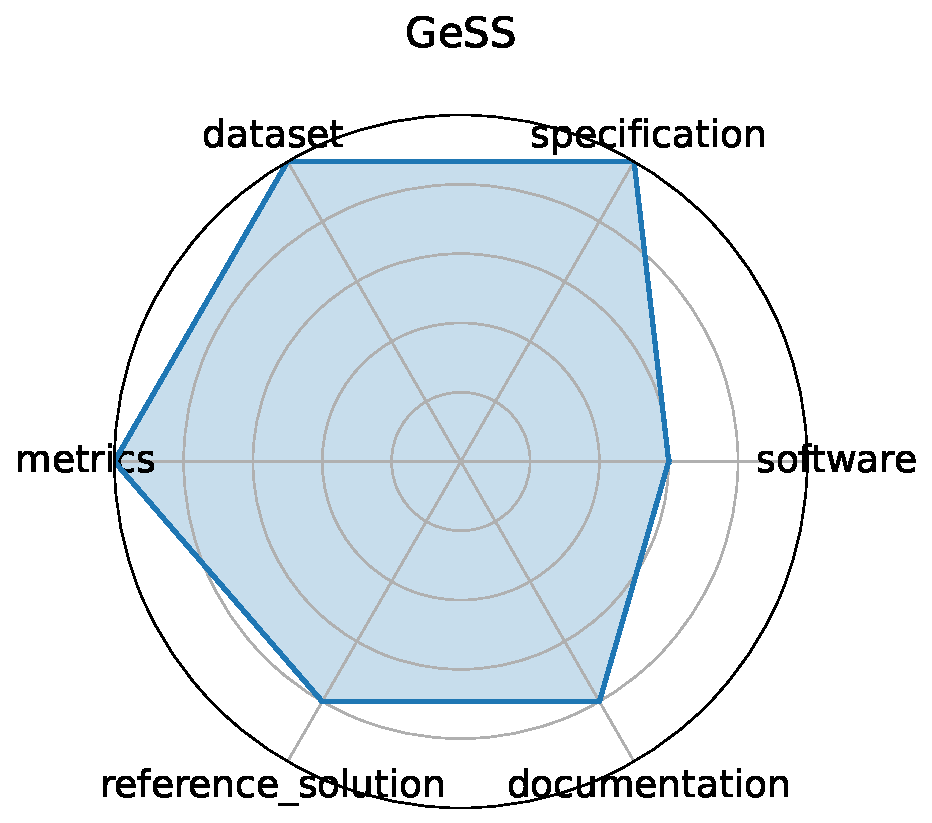
\includegraphics[width=0.2\textwidth]{gess_radar.pdf}
}}
\clearpage